\chapter{Lighting and rendering}
\label{ch:light}

\section{Lights, the world and the views}
Lights are Directional, Point, Spot and Area, with an optional colour temperature in kelvin \cite{Kang2002Design};
\ui{Aim at Point} turns a light to shine at the surface you click. The Scene and Game views rasterize (deferred PBR with
sun shadows and image-based lighting), so editing stays fast. The world is a gradient, Blender's Hosek--Wilkie
physical sky \cite{Hosek2012Analytic} driven by the first Directional Light, an HDRI or a colour, with a sun disc, a
horizon band and distance fog; the view transforms are Standard, Filmic, ACES, Unity's ACES (the curve Unity's
post-processing applies \cite{Hill2016ACES}) and, with OpenColorIO, AgX and Blender's others. The sky, fog and ambient
light are edited in one place, the \textbf{Lighting} window.

\section{F12 and the Render window}
\key{F12} renders the active camera with either engine: \textbf{rasterized} with supersampling, or \textbf{path traced}
(Cycles-like: soft shadows, bounced light, glass, fog, depth of field, with Embree and OpenImageDenoise when Blender's
libraries are present, else Blendity's own BVH and \`A-Trous denoiser). The \textbf{Render} window (\key{F11}) has
resolution presets, the device (CPU, GPU Compute on any Vulkan GPU, OptiX on NVIDIA, or GPU + CPU together: path tracing
picks the faster device by itself and never overruns a small GPU's memory), samples, path guiding, Film $>$
Transparent, and saves PNG, JPEG, HDR or EXR. \ui{Render Camera Sequence} renders every camera marked In Sequence;
\ui{Render Animation} (\key{Ctrl+F12}) renders every frame of the sequence or the selected clip as numbered PNGs and an
H.264 MP4 beside them (ProRes and a VRChat-ready preset too; the dependency-free build offers Blender's libraries or an
\code{ffmpeg} on the PATH); \ui{Live Preview} re-renders a quick preview as you edit; the image pans with a left drag.
MoonRay, DreamWorks' renderer \cite{MoonRay2026}, is an optional download run as a program of its own.

\begin{figure}[H]
  \centering
  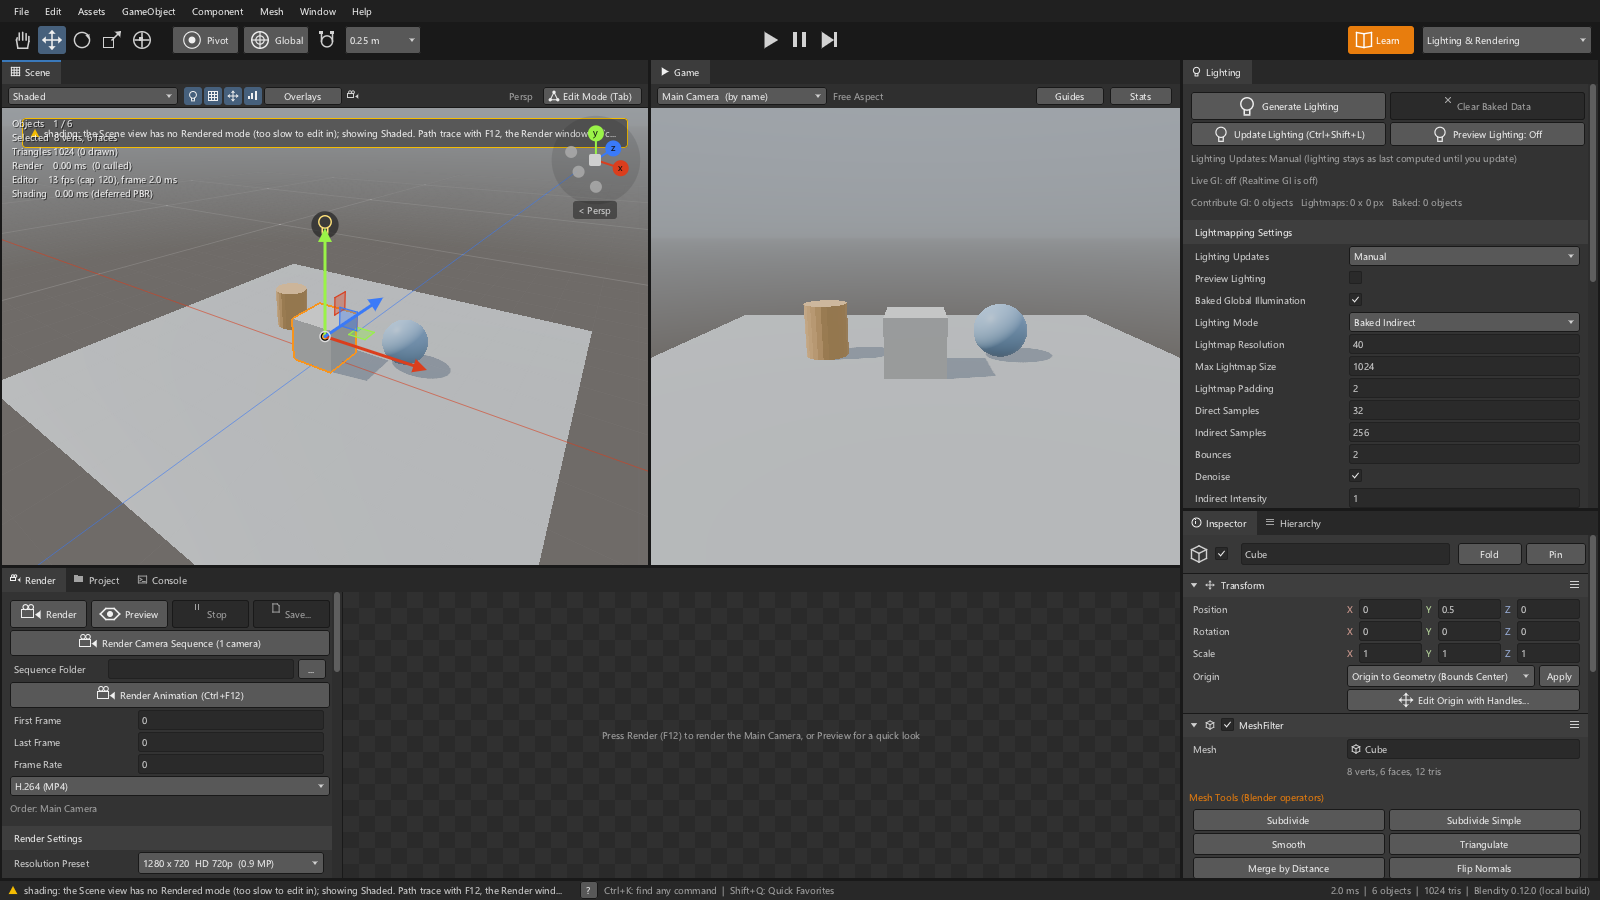
\includegraphics[width=\textwidth, alt={The Lighting and Rendering layout: the Scene view and the Game view side by side, the Lighting window with Generate Lighting and the lightmapping settings on the right, the Render window with its presets along the bottom.}]{layout-lighting.png}
  \caption{The Lighting \& Rendering layout: the Scene view, the Game view through the Main Camera, the Lighting
  window (Generate Lighting, the lightmapping settings) and the Render window with its presets.}
\end{figure}

\section{Baked, mixed and realtime light}
The short version for a scene that doesn't lag, as Unity does it \cite{UnityManual2026}:
\begin{enumerate}
  \item \textbf{Static objects:} select everything that never moves and tick \ui{MeshRenderer > Contribute GI}
    (\ui{Mark Static Meshes} does it for a world). Lightmap UVs are made for you.
  \item \textbf{Lights:} set each light's \ui{Mode}: \emph{Baked} (everything baked), \emph{Mixed} (bounces baked, direct
    light and shadows live: the usual choice for the sun) or \emph{Realtime}.
  \item \textbf{Bake:} \menu{Window > Lighting > Generate Lighting}. A baked lightmap costs about 1~ms on a 1080p frame.
  \item \textbf{Moving objects} take their bounced light from a \ui{Probe Volume} component (add one and bake again);
    metal and glass reflect a \ui{Reflection Probe}'s cubemap inside its box.
  \item \ui{Auto Generate} bakes again a second after you stop editing; the status bar says ``Lighting out of date''
    until it does. The bake is saved next to the scene.
\end{enumerate}
\ui{Lighting Updates: Manual} (the default) keeps bounced light as last computed while you drag things; \ui{Update
Lighting} (\key{Ctrl+Shift+L}) refreshes it; \ui{Preview Lighting} shows a rough bake half a second after you stop.
\textbf{Realtime GI} (voxel global illumination \cite{Thiedemann2011Voxel}) shows bounced light while you're still
arranging, with nothing to bake, and runs 4 to 8 times faster on a Vulkan GPU; set Render $>$ Device to GPU Compute
and Generate Lighting bakes on the GPU too.

\begin{center}
\small
\begin{tabularx}{\textwidth}{lXX}
\toprule
Setting & What it does & When to change it \\
\midrule
Lightmap Resolution & texels per metre (Unity's default is 40) & lower for big scenes, higher for sharp contact shadows \\
Indirect Samples, Bounces & rays per texel; how many times light bounces & raise if noisy; 3 or 4 for interiors \\
GI Resolution, Realtime Resolution & the live GI's share of the screen; realtime lightmaps' texels per metre & Half for a cleaner Scene view; higher for small rooms \\
Indirect Intensity & scales the baked bounce & artistic control \\
GI Device, Voxel Resolution & where realtime GI gathers; 64, 128 or 256 voxels across the scene & CPU only to compare; higher for small detail \\
Probe Min / Max Spacing & probe density near geometry / in open space & lower min spacing for small rooms \\
\bottomrule
\end{tabularx}
\end{center}

\section{Camera filters}
Camera filters are Unity's post-processing stack as components on a camera (\ui{Add Component > Camera Filters},
then \ui{Add Filter}): colour grading, bloom, vignette, chromatic aberration, lens distortion, film grain, CRT,
pixelate, edge outline, sharpen, halftone, hatching, line art, paper, a colour ramp, and whole looks: \textbf{Retro
Console} (PlayStation, N64, Saturn, DOS: wobbling vertices, affine textures, dithered colour \cite{psxspx}) and
\textbf{Anime / Manga}. They show in the Game view, the Camera Preview, F12 (traced renders too) and camera sequences;
the Scene view can look through them.

\begin{example}{a PS1-style render}
\begin{enumerate}
  \item Select the camera, \ui{Add Component > Camera Filters}, \ui{Add Filter > Retro Console}, Console: PlayStation.
  \item \key{F12}: the wobbling vertices, affine textures and dithered colour show in the path-traced render too.
\end{enumerate}
\end{example}

\section{Developing a render: the Editing tab}
\menu{Window > Editing} (or the Editing layout) develops a render or an image the way Lightroom does: a stack of
adjustments (Exposure, Contrast, Highlights / Shadows, white balance, a Tone Curve, HSL, Clarity, Dehaze, Sharpen,
Noise Reduction, Vignette, Crop), each limited by a mask if you like (a gradient, a tone or colour range, a brush),
applied in linear light and never written into the source: \ui{Save} keeps the stack beside the image, \ui{Export}
writes the result, \ui{Use as Camera Look} gives the camera the same look live, \ui{Apply to Texture} puts an edit on a
texture.

\section{A scene opened from Unity}
A Unity scene opened here looks as its Game view does: its fog mode, skybox, camera flags, post-processing (the ACES
tonemapper, exposure, grading, bloom, vignette), the lights' shadows and cookies, its reflection probes, and Unity's own
baked lightmaps and light probes (\ui{Lighting > Use Unity's Lightmaps}, read by your installed Unity in the
background). The match is measured station by station against Unity's renders (\code{docs/hci/compare-unity-vrchat-2026-11.md}).

\begin{fromnote}{Where it comes from}
The rasterizer follows EEVEE and the path tracer Cycles \cite{Blender2026}; the lighting modes, lightmaps, probe
volumes and post-processing follow Unity \cite{UnityManual2026}; the physical sky is Hosek and Wilkie's
\cite{Hosek2012Analytic}; realtime GI is Thiedemann et al.'s \cite{Thiedemann2011Voxel}; the microfacet model and
its sampling are Cook--Torrance, Walter et al.\ and Heitz \cite{Cook1982Reflectance, Walter2007Microfacet,
Heitz2018Sampling}; the denoiser is Dammertz et al.'s \cite{Dammertz2010Edge}; path guiding is Ruppert et al.'s
\cite{Ruppert2020Robust}; the bloom is Jimenez's \cite{Jimenez2014}; the theory is in \cite{MarschnerShirley2021}
(ray tracing, Monte Carlo, tone reproduction) and \cite{Gregory2018vol2} (lighting, post-processing). Learn: \emph{How
This Editor Renders}, \emph{Lights and Materials}, \emph{Render Engines}, \emph{Light, Sky and Tone Mapping},
\emph{Baked and Realtime Lighting}, \emph{Rendering on the GPU}, \emph{Editing: Develop a Render}.
\end{fromnote}
